\section{实验结果与分析}
本次实验比较特殊,仅通过仿真即可完成实验结果的正确性检测。

\subsection{仿真代码设计}
为了验证各项功能与各种情况的正确性,我组使用了如下仿真代码

\begin{lstlisting}[language = {verilog}]
module cache_sim;

// Inputs
reg clk;
reg rst;
reg [31:0] addr;
reg load;
reg store;
reg edit;
reg invalid;
reg [2:0] u_b_h_w;
reg [31:0] din;

// Outputs
wire hit;
wire [31:0] dout;
wire valid;
wire dirty;
wire [22:0] tag;

// Instantiate the Unit Under Test (UUT)
cache uut (
	.clk(~clk), 
	.rst(rst), 
	.addr(addr), 
	.load(load),
	.store(store), 
	.edit(edit), 
	.invalid(invalid), 
	.u_b_h_w(u_b_h_w),
	.din(din), 
	.hit(hit), 
	.dout(dout), 
	.valid(valid), 
	.dirty(dirty), 
	.tag(tag)
);

initial begin
	clk = 1;
	forever #10 clk = ~clk ;
end

reg [31:0]counter = 0;

always @(posedge clk) begin
	counter <= counter + 32'b1;

	case (counter)
		// Initialize Inputs
		32'd0: begin
			rst <= 0;
			addr <= 0;
			load <= 0;
			store <= 0;
			edit <= 0;
			invalid <= 0;
			u_b_h_w <= 0;
			din <= 0;
		end

		// init
		32'd10: begin
			load <= 0;
			store <= 1;
			edit <= 0;

			din <= 32'h11111111;
			addr <= 32'h00000004;
		end

		32'd11: begin
			addr <= 32'h0000000C;
		end

		32'd12: begin
			addr <= 32'h00000010;
		end

		32'd13: begin
			addr <= 32'h00000014;
		end

		// read miss
		32'd14: begin
			load <= 1;
			store <= 0;
			edit <= 0;

			u_b_h_w <= 3'b010;
			din <= 0;
			addr <= 32'h00000020;
		end

		// read hit
		32'd15: begin
			u_b_h_w <= 3'b010;
			addr <= 32'h00000010;
		end

		// write miss
		32'd16: begin
			load <= 0;
			store <= 0;
			edit <= 1;

			u_b_h_w <= 3'b010;
			din <= 32'h22222222;
			addr <= 32'h000000024;
		end

		// write hit
		32'd17: begin
			u_b_h_w <= 3'b010;
			addr <= 32'h00000014;
		end


		// read line 0 of set 0, set recent bit
		32'd18: begin
			load <= 1;
			store <= 0;
			edit <= 0;

			u_b_h_w <= 3'b010;
			din <= 0;
			addr <= 32'h00000004;
		end

		// store to line 1 of set 0 due to line 0 recent
		32'd19: begin
			load <= 0;
			store <= 1;
			edit <= 0;

			u_b_h_w <= 3'b010;
			din <= 32'h33333333;
			addr <= 32'h00000204;
		end

		// edit line 1 of set 0, set dirty & recent
		32'd20: begin
			load <= 0;
			store <= 0;
			edit <= 1;

			u_b_h_w <= 3'b010;
			din <= 32'h44444444;
			addr <= 32'h00000204;
		end

		// read line 0 of set 0, set recent bit
		32'd21: begin
			load <= 1;
			store <= 0;
			edit <= 0;

			u_b_h_w <= 3'b010;
			din <= 0;
			addr <= 32'h00000004;
		end

		// read miss, tag mismatch. output tag (of line 1), valid and dirty == 1
		32'd22: begin
			load <= 1;
			store <= 0;
			edit <= 0;
			
			u_b_h_w <= 3'b010;
			din <= 32'h0;
			addr <= 32'h00000404;
		end

		// auto replace line 1 of set 0
		32'd23: begin
			load <= 0;
			store <= 1;
			edit <= 0;

			u_b_h_w <= 3'b010;
			din <= 32'h55555555;
			addr <= 32'h00000404;
		end

		// clear
		default: begin
			load <= 0;
			store <= 0;
			edit <= 0;
			din <= 0;
			addr <= 0;
		end
	endcase
end

endmodule    
\end{lstlisting}

\subsection{仿真结果分析}

根据仿真代代码,我们组对仿真结果的详细分析如下所示:首先我们需要对整个cache进行初始化,
清空所有缓存并重置所有控制信号,这个过程持续十个周期
\begin{figure}[H] %H为当前位置,!htb为忽略美学标准,htbp为浮动图形
	\centering %图片居中
	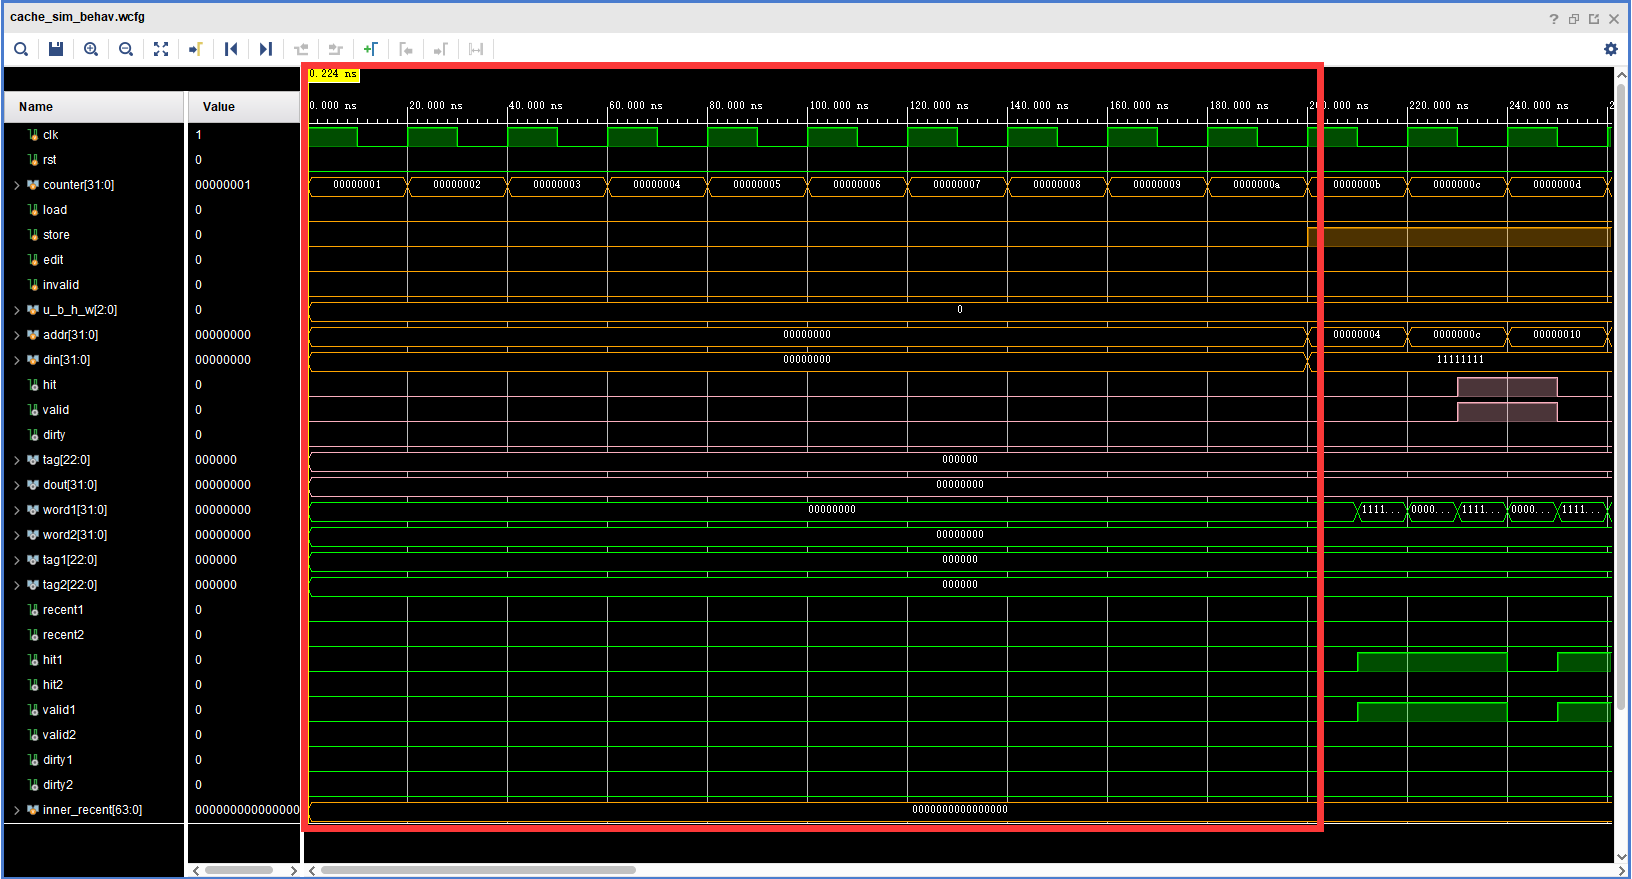
\includegraphics[width=1.0\textwidth]{figs/res1.png} %插入图片,[]中设置图片大小,{}中是图片文件名
	\caption{初始化过程} %最终文档中希望显示的图片标题
	\label{Fig.2} %用于文内引用的标签
\end{figure}

\subparagraph{Store实现Cache的初始化}
状态初始化之后,首先验证store的正确性,
首先输入的数据为32'h11111111,地址为32'h00000004,此时hit信号为0,说明是写缺失。
然后紧接着保持需要写入的数据不变,将写入地址改为32'h0000000C,此时我们可以发现32'h0000000C的Index与Tag均与32'h00000004相同,仿真结果上hit信号也升起,结果正确。
继续保持写入数据不变,将写入地址改为32'h00000010,此时Index与cache中的已经写入的Data Line均不同,hit信号没有升起,Cache将对应块读入。
最后将写入地址改变为32'h00000014此地址对应的Data Line与32'h00000010相同,故又会产生hit信号,仿真结果正确。
至此,Cache的Index为0, 1的两个Data Line都被填满。

\begin{figure}[H] %H为当前位置,!htb为忽略美学标准,htbp为浮动图形
	\centering %图片居中
	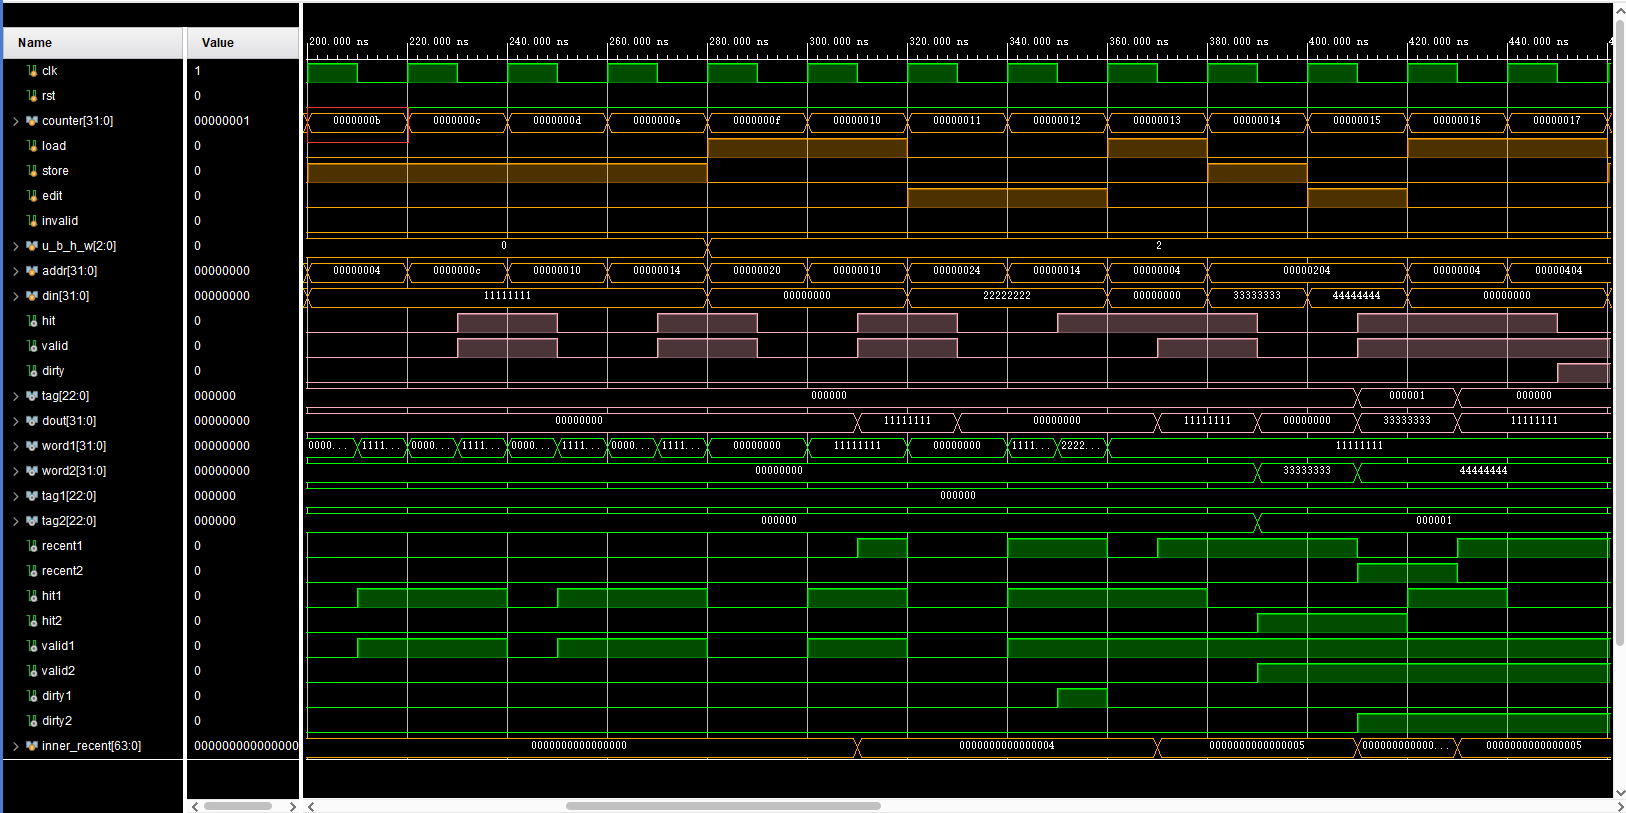
\includegraphics[width=1.0\textwidth]{figs/res2.png} %插入图片,[]中设置图片大小,{}中是图片文件名
	\caption{Store过程} %最终文档中希望显示的图片标题
	\label{Fig.3} %用于文内引用的标签
\end{figure}

\subparagraph{Read验证}
通过上述过程,Cache已经被初始化完毕,我们写下来验证read miss的情形,我们采用load读取
32'h00000020地址所对应的一个Word的形式来验证,32'h00000020的Index为2,
会产生read miss,hit信号没有升起。
在下一个周期,当我们读取32'h00000010的一个Word时,会发现Index为1的Data Line中有Tag为0的Data Line,
此时hit信号升起,并且Tag位0的数据块由于产生了读取操作,属于最近被访问,它的recent位会被置为1,与之对应的另一Data Line的recent位被置为0
从仿真图的对应位置来看,仿真结果正确。

\begin{figure}[H] %H为当前位置,!htb为忽略美学标准,htbp为浮动图形
	\centering %图片居中
	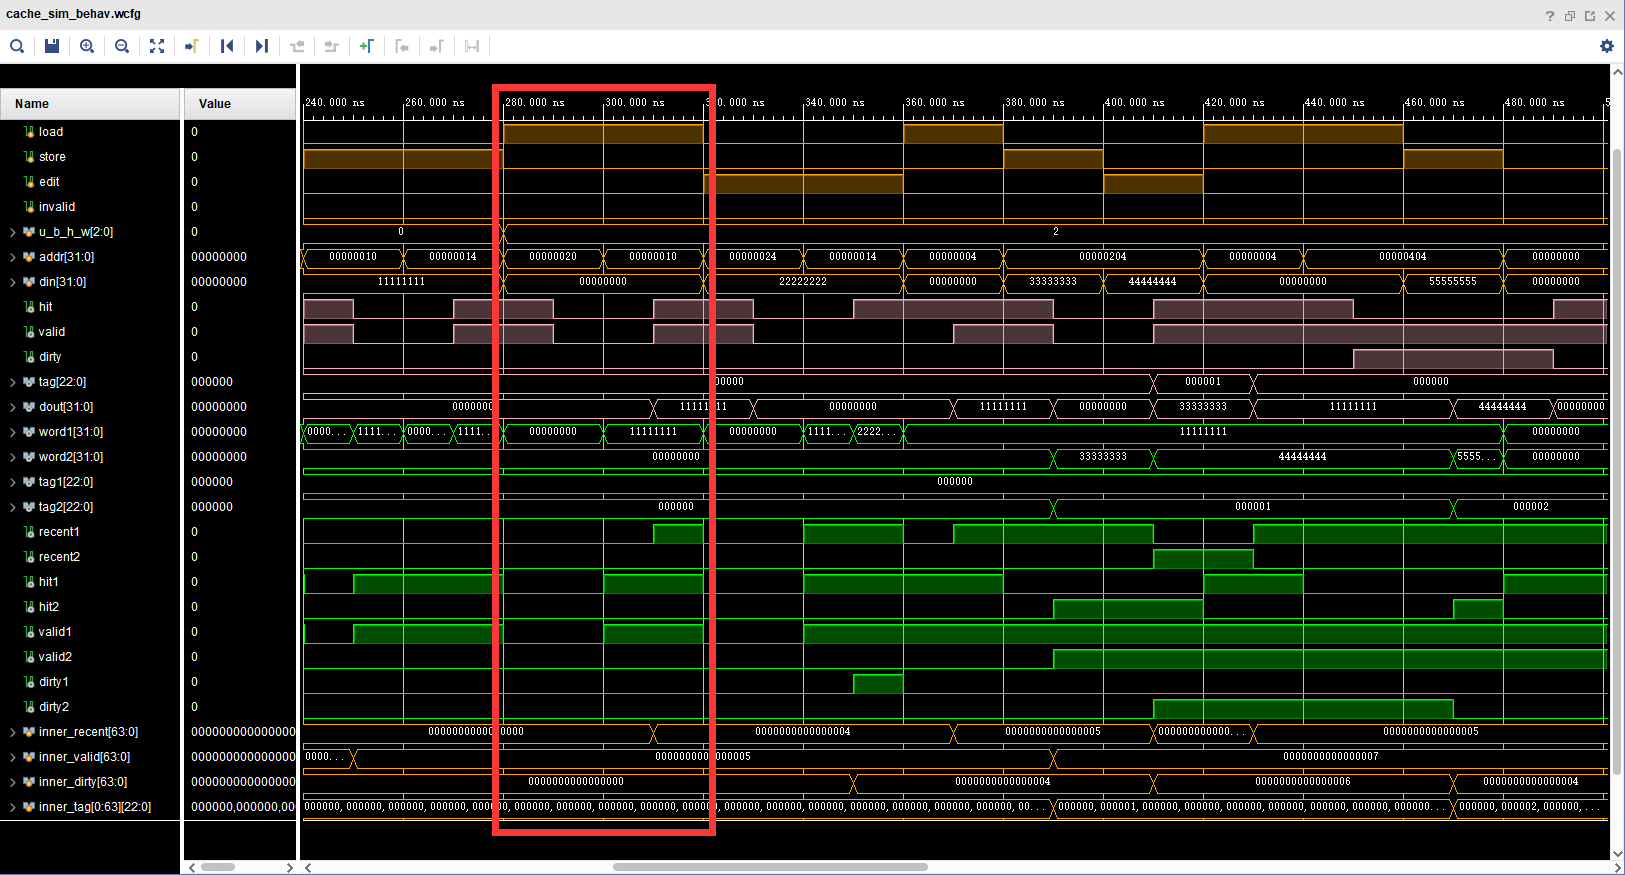
\includegraphics[width=1.0\textwidth]{figs/res3.png} %插入图片,[]中设置图片大小,{}中是图片文件名
	\caption{Read过程} %最终文档中希望显示的图片标题
	\label{Fig.4} %用于文内引用的标签
\end{figure}

\subparagraph{Write验证}
下面我们继续来验证Write操作的正确性,同样通过Write hit与Write Miss两种情形分别验证,首先我们使用edit
向地址为32'h000000024的地方修改一个数据,此时Index为2,显然是Miss的,此时hit信号没有升起,结果正确。
但需要修改的地址为32'h00000014时,由于前面的读写操作,此地址对应的数据块应该加载进了Cache中,所以此时hit信号会升起
同时我们可以直到是两路中的第一路命中,命中产生修改之后,此块的recent位与Dirty位都会被置为1,说明它最近被修改过。

\begin{figure}[H] %H为当前位置,!htb为忽略美学标准,htbp为浮动图形
	\centering %图片居中
	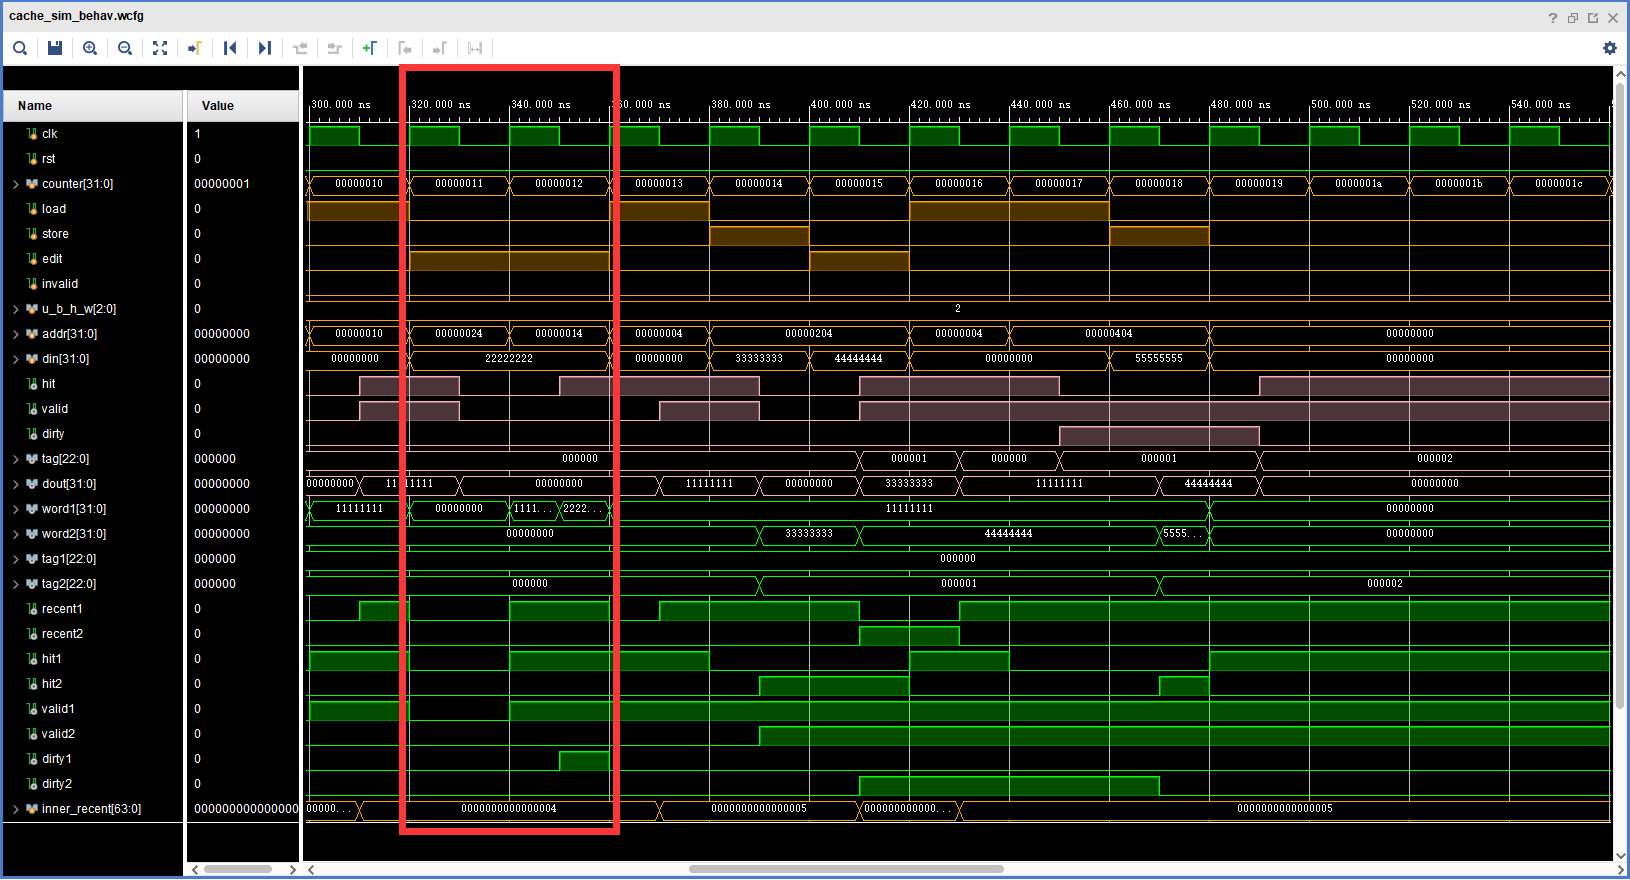
\includegraphics[width=1.0\textwidth]{figs/res4.png} %插入图片,[]中设置图片大小,{}中是图片文件名
	\caption{Write过程} %最终文档中希望显示的图片标题
	\label{Fig.5} %用于文内引用的标签
\end{figure}

\subparagraph{Cache Mode验证}
下面的过程会通过一系列读写操作完成对本次实验中使用到的Cache Mode进行验证,主要验证
LRU替换策略,Write Back与Write Allocate策略。

首先使用ld指令读取地址为32'h00000004的一个word,显然是Hit的,并且这一操作会使此数据块(line 0)被设置为最近使用。
再使用store指令写入到32'h00000204,此时会将此地址的数据块读入到set 0,但是由于line 0的recent位为1,
说明最近被使用,所以会直接store到的line 1,并且是写失效。
下个周期修改地址为32'h00000204的Word,此时line 1被修改,Dirty位与Recent位均被置为1,line 0的recent位被置为1为0,从仿真结果来看正确。
然后再通过read操作读取一个line 0,使其成为最近访问的Data Line。
然后再读取32'h00000404的数据块,此时由于tag位与两个Data Line均不匹配,会发生read miss。
最后写入内容32'h00000404,发生write miss,并且由于LRU策略此时line 1是需要被替换的那一块,而line 1又是有效并且Dirty的,所以line 1会被写回内存,从仿真图来看结果正确。

\begin{figure}[H] %H为当前位置,!htb为忽略美学标准,htbp为浮动图形
	\centering %图片居中
	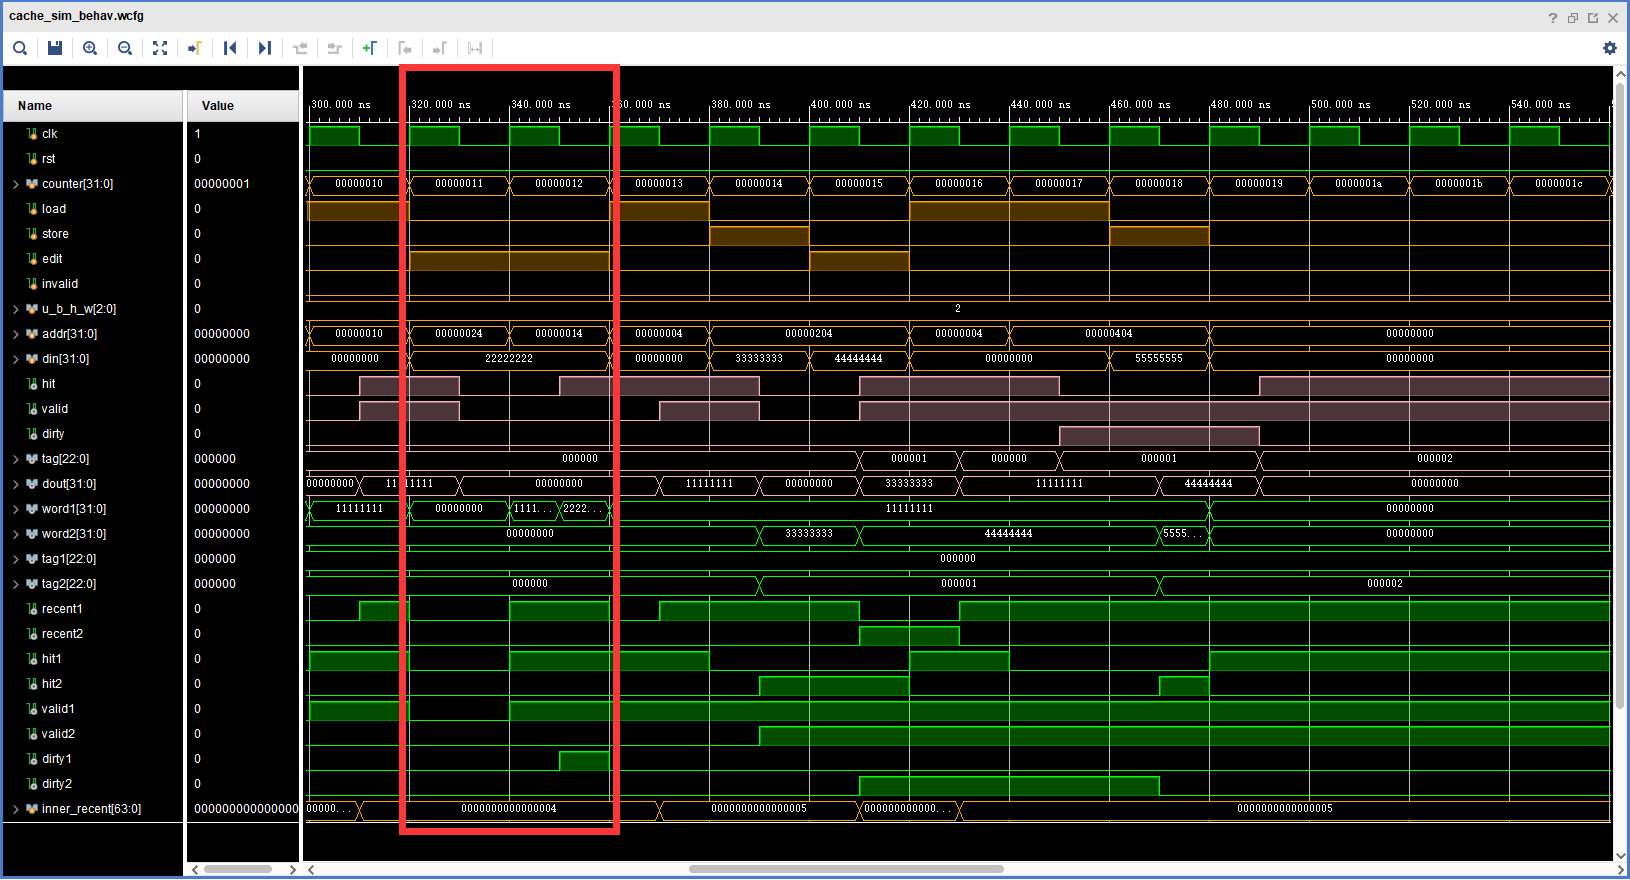
\includegraphics[width=1.0\textwidth]{figs/res4.png} %插入图片,[]中设置图片大小,{}中是图片文件名
	\caption{Write过程} %最终文档中希望显示的图片标题
	\label{Fig.5} %用于文内引用的标签
\end{figure}